\section{System Architecture}
\label{sec:system}

\begin{figure*}[t]
\centering
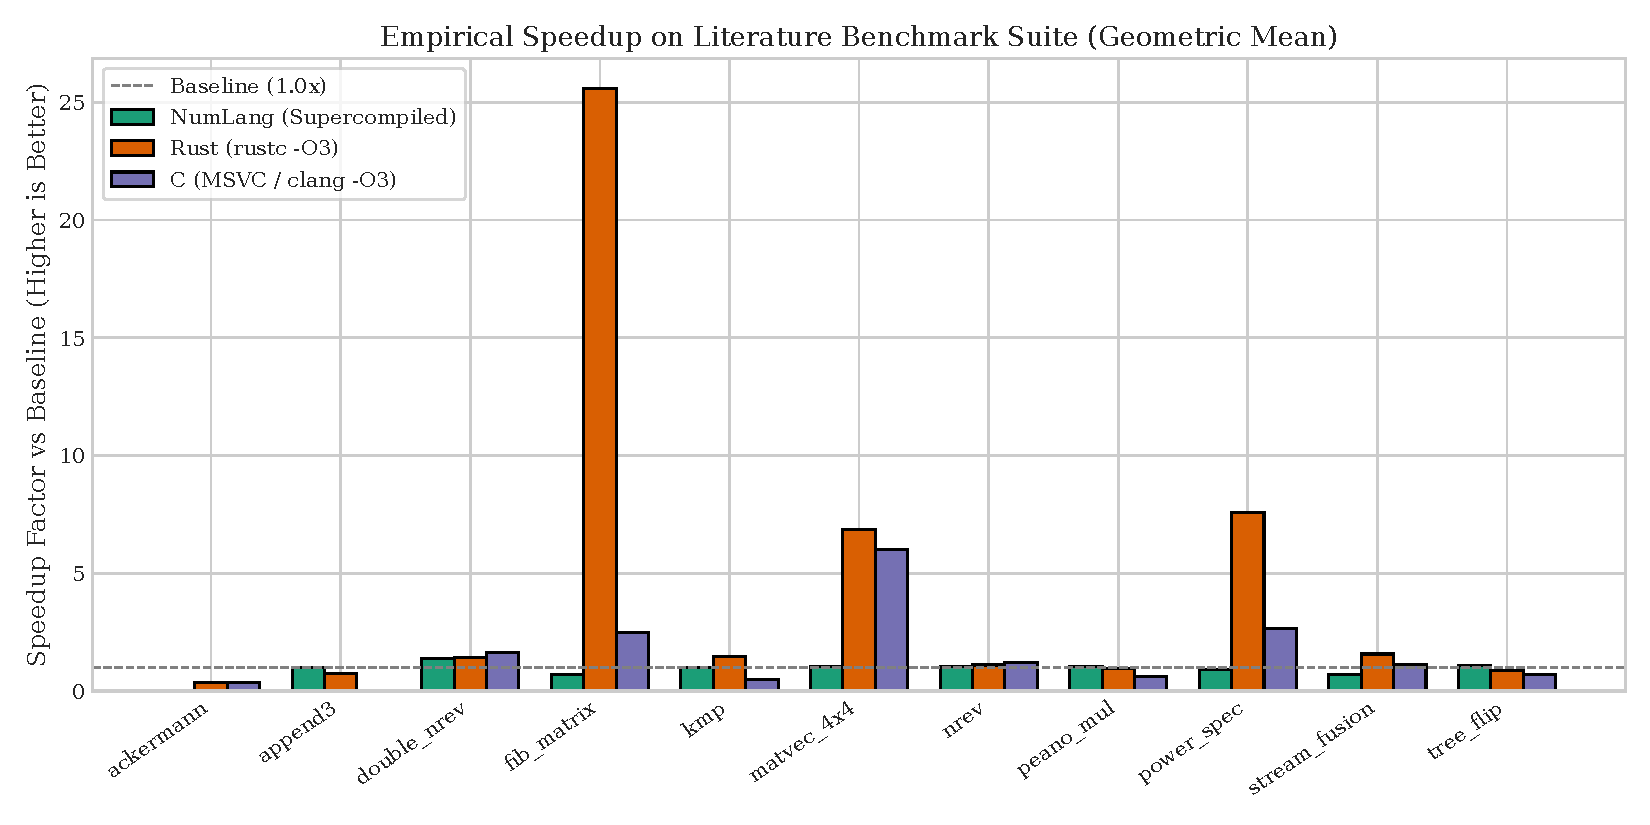
\includegraphics[width=0.92\textwidth]{figures/architecture.pdf}
\caption{The end-to-end NumLang compilation pipeline: from high-level source text to verified native binaries through the SSA process-tree supercompiler.}
\label{fig:architecture}
\end{figure*}

NumLang is structured as a multi-stage compilation pipeline where supercompilation acts as a central mid-level optimizing transformation. Figure~\ref{fig:architecture} depicts the end-to-end system flow.

\subsection{Pipeline Overview}
The compiler operates in seven sequential stages:
\begin{enumerate}
    \item \textbf{Parsing \& Typechecking}: Source code (\texttt{.nl}) is tokenized and parsed into an AST, followed by bidirectional type inference and check.
    \item \textbf{MIR Lowering}: Typed ASTs are lowered into Static Single Assignment (SSA) form with basic blocks, MemorySSA tokens, and explicit $\phi$-functions.
    \item \textbf{Process-Tree Driving}: The symbolic driving engine executes the MIR with abstract inputs, maintaining path constraints and a symbolic heap.
    \item \textbf{Distillation \& MRSC}: The engine searches an MRSC hypergraph, folding global configurations and applying Hamilton distillation to deforest cross-boundary data flows.
    \item \textbf{Refinement \& Compaction}: Interval refinement narrows loop bounds and eliminates bounds checks; post-distillation compaction removes dead configurations and redundant bindings.
    \item \textbf{Cache Validation}: Specialization candidates are queried against the content-addressed disk cache; misses are validated and saved.
    \item \textbf{Native Codegen}: Residualized MIR functions are lowered to standalone native binaries via Cranelift or LLVM.
\end{enumerate}

\subsection{Module Breakdown}
\paragraph{Lexer and Pratt Parser.}
The lexer handles structured tokens, arithmetic and bitwise operators, and keyword identification. The parser implements top-down operator precedence (Pratt parsing) to generate an untyped AST supporting functions, recursive types, let-bindings, loops, and first-class closures.

\paragraph{Bidirectional Typechecker.}
The typechecker verifies type correctness, polymorphic instantiations, and immutability invariants. It guarantees that all function signatures, local variable types, and closure capture environments are fully resolved before lowering.

\paragraph{MIR Lowering and Mem2Reg Pass.}
The lowering pass transforms the AST into a linear control-flow graph. Local variables allocated on the stack are promoted to pure SSA values via iterated dominance frontiers (Mem2Reg), producing explicit $\phi$-nodes and canonicalizing loop headers.

\paragraph{Positive Symbolic Execution Driver.}
The driver maintains a \texttt{SymbolicState} mapping SSA registers to hash-consed symbolic terms (\texttt{SymTerm}). Statements are evaluated abstractly: branch conditions fork the process tree and attach path constraints to child configurations, pruning infeasible paths immediately.

\paragraph{Topological Whistle \& Homeomorphic Embedding.}
To guarantee termination, every newly generated configuration is checked against all ancestors along its process-tree spine using the homeomorphic embedding relation $\trianglelefteq$. If an ancestor embeds into the current state, the whistle halts expansion and triggers generalization or knot tying.

\paragraph{Textbook Anti-Unification (MSG) \& Knot Remapping.}
When a whistle fires, the generalization engine computes the Most Specific Generalization (MSG) between the ancestor and current configuration following Sørensen and Glück~\cite{sorensen1995algorithm}. Common subterms are preserved while divergent subterms are abstracted into fresh symbolic variables. The residualizer emits parallel state transfers and re-maps $\phi$-node basic block IDs on back-edges.

\paragraph{Hamilton Global Distillation Engine.}
Unlike local supercompilers that only fold configurations within a single function body, NumLang's distillation engine tracks configurations across distinct call sites and function boundaries, folding nested compositions (such as \texttt{append3}) into a single recursive pass.

\paragraph{MRSC Hypergraph Explorer.}
NumLang implements Multi-Result Supercompilation (MRSC)~\cite{klyuchnikov2012practical}. Rather than committing greedily to a single generalization strategy, the explorer constructs a configuration hypergraph representing alternative driving, folding, and generalization choices, extracting the Pareto-optimal residual program under a user-defined cost metric.

\paragraph{Refinement Type Engine.}
Path constraints collected along process-tree branches are translated into numerical intervals $[L, U] \subseteq \mathbb{Z}$. The refinement engine narrows intervals across arithmetic operations and comparisons, statically identifying unreachable branches and redundant array bounds checks.

\paragraph{Post-Distillation Compaction.}
Before code generation, the process tree is compacted by pruning dead overflow configurations and merging alpha-equivalent knot targets. A subsequent MIR peephole pass applies copy propagation and $\eta$-reduction to eliminate identity assignments and intermediate registers.

\paragraph{Cross-Module Specialization Cache.}
To avoid re-supercompiling unchanged functions, NumLang implements a content-addressed disk cache. Each specialization key is computed via a SHA-256 hash over the function's normalized MIR body, argument types, and symbolic constraints. Cache entries use a two-level hex directory fanout, achieving up to $10\times$ compilation speedups on warm rebuilds.

\paragraph{Translation Validation \& SMT Oracle.}
Before native code emission, the supercompiled MIR is verified against the original unspecialized MIR using an integrated SMT translation validator. The validator formulates relational verification conditions across all path pairs and dispatches them to an SMT solver (Z3) to confirm bisimulation equivalence.

\paragraph{Native Codegen (Cranelift / LLVM).}
Validated MIR functions are lowered to native machine instructions. NumLang supports both Cranelift (for ultra-fast debug compilation) and LLVM (for maximum runtime optimization and vectorization), producing standalone static executables.
